\section{The Nyquist Stability Criterion}

\subsection{Frequency response}
The frequency response of a system is the steady-state response of a system to a sinusoidal input.
The output of a time-invariant system will have the same frequency as the sinusoidal input,
but possibly with a different amplitude and phase.

The output of a time-invariant system is given by:
$$y(t) = \int_{-\infty}^{\infty} h(\tau)u(t-\tau)d\tau$$
Where y is the output, u  is the input, and h is the impulse response of the system.

To obtain the frequency response, only sinusoidal inputs are considered.

The frequency response of H(s) is given by the magnitude and phase of $H(j\omega)$

$$M = |H(j\omega)|$$
$$\phi = \angle H(j\omega)$$
The M is the amplitude ratio and $\phi$ is the phase shift.

The system response to the input $u(t) = cos(\omega t)$ is given by:
$$y(t) = \frac{A}{2} M(\omega) cos(\omega t + \phi(\omega))$$

This explains why the output will have the same freqency as the input, but possibly with a different amplitude and phase.

The bandwidth of a closed-loop system $T(s)$ is defined to be the maximum frequency at which
the output y of a system will track a sinusoidal input $r$ in a satisfactory manner. Output attaenuated to $1/\sqrt{2}$ of the input amplitude.
Formally the bandwidth $\omega_{BW}$ of $T(s)$ is the maximal frequency such that:

$$T(j\omega) >= 1/\sqrt{2}$$

The maximal value of the frequency response is called the resonant peak,

\begin{center}
	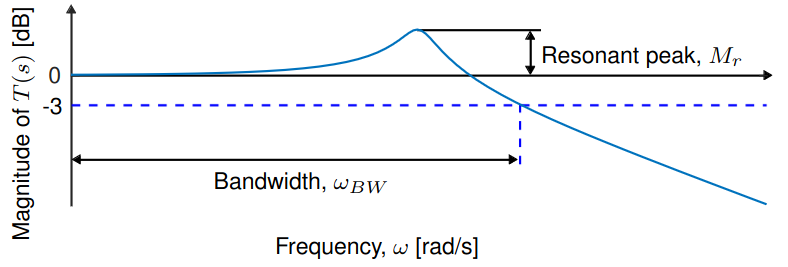
\includegraphics[width=0.8\textwidth]{Images/resonantPeak.png}
\end{center}

\newpage

\subsection{Bode Plots}
Pole decreases the magnitude of the frequency response by 20dB/decade.
Zero increases the magnitude of the frequency response by 20dB/decade.

\textbf{Bode Form of transfer function}

In the follwing, we consider the open-loop transfer function
$$KG(s) = K  \frac{(s-z_1)(s-z_2)\cdots}{(s-p_1)(s-p_2)\cdots}$$
For convenience, the transfer function is evaluated at $s = j\omega$ and rewritten into
Bode form as follows:
$$ KG(j\omega) = K_0 \frac{(j\omega \tau_1 +1)(j\omega \tau_2 +1)\cdots}{(j\omega \tau_a+1)(j\omega \tau_b +1)\cdots}$$

\textbf{Classes of terms in transfer function}

\textbf{Class 1:} $K_0(j\omega)^n$ for $n\in \mathbb{Z}$

If $n>0$ then the term is a zero at the origin. If $n<0$ then the term is a pole at the origin.
It can be more than one depending on the value of n.


Example: For the term $K_0(j\omega)^n$ we have:
$$ log K_0 |(j\omega)| = log K_0 + n log \omega$$
This means that the magniutde plot is a straight line with slope $n \cdot (20 dB/dec)$
The phase of $(j\omega)^n$ is constant and given by: $\phi = n \cdot 90^{\circ}$

If $n=-1$, this means that there is a pole at the origin. This therefore leads to a slope of $-20 dB/dec$ and a phase shift of $-90^{\circ}$

\textbf{Class 2:} $(j\omega \tau + 1)^{\pm1}$

real pole or zero.


For $\omega \tau << 1, j\omega \tau \approx 1$

For $\omega \tau >> 1, j\omega \tau + 1 \approx j\omega \tau$

In addition, for $\omega = 1/\tau$, the gain is $\sqrt{2}$ - an increase of 3dB compared to the DC gain.
The point $\omega = 1/\tau$ is called the break point. At the break point the angle is $45^{\circ}$.
Thus, the phase changes from a decade before the brake point to a decade after the break point.

\textbf{Class 3:} $((j\omega / \omega_n)^2 + 2\zeta (j\omega / \omega_n) + 1)^{\pm1}$

Complex conjugate poles or zeros.


For $\omega << \omega_n$, the amplitde is approximately 1.
In addition, at the break point $\omega = \omega_n$, the magnitude is $|G(j\omega)| = 1/(2\zeta)$
and the phase is $\pm90^{\circ}$


\textbf{Summary of Bode Plot Rules}

\begin{enumerate}
	\item{Rewrite the considered transfer function to bode form}
	\item{Determine the value of the $K_0(j\omega)^n$ term. Plot the low frequency magnitude
	            asymptote through the point $K_0$ at $\omega = 1$ and with slope of $n \cdot 20 dB/dec$}
	\item{Complete the composite magnitude asymptotes by extending the low-frequency
	            asymptote until the first frequency break point. Then change the slope according to
	            the behavior at the break point, and continue the procedure for the remaining break points.}
	\item{Sketch the approximate magnitude curve by increasing the asymptote value by a factor $\sqrt{2}$ at first-order numerator
	            break and decreasing it by a factor $1/\sqrt{2}$ at denominator break.}
	\item{Plot the low-frequency asymptote  of the phase $phi=n \cdot 90^{\circ}$}
	\item{Change the phase at the phase points, and correct the phase according to the slope
	            at the phase point.}
\end{enumerate}

\subsection{Nyquist Stability Criterion}

Nyquist can be used for open-loop unstable systems, whereas you can't use bode plots.
But you must know the open loop poles in order to determine the number of
closed-loop zeros in the right half plane.


A contour map of a complex function will encircle the origin Z-P times where Z is the number
of zeros and P is the number of poles of the function inside the contour.

To verify the stability of a system, one needs to determine the number of closed-loop poles
in the right halp plane. Thus, the Nyquist plot is a map of a contour that encircles
the entire right-half plane.

The number of closed-loop poles in the right half-plane equals the number of right half-plane
zeros of the characteristic equation. The characteristic equation is given by:
$$1+KG(s) = 0$$

Let N denote the number of clockwise encirclements of -1. Then the number of zeros in
the right half plane Z (closed-loop poles) minus the number of open-loop poles in the right half plane P.
$$N = Z-P$$

\textbf{Steps}

\begin{enumerate}
	\item Nyquist plot of $KG(j\omega)$
	\item Determine the number of encirclements of -1 and note direction
	\item Figure out how many more poles or zeros are in the right half plane.
\end{enumerate}




\subsection{Examples}
